\documentclass[12pt,aspectratio=169]{beamer}

% Input
\usepackage[utf8]{inputenc}
\usepackage[T1]{fontenc}
\usepackage[letterspace=100]{microtype}
\usepackage{upquote}

% Beamer
\usetheme{metropolis}
\usepackage[sfdefault]{FiraSans}
\usepackage{xcolor}
\definecolor{blue}{HTML}{002957}
\definecolor{red}{HTML}{F1563F}
\setbeamercolor{palette primary}{fg=white,bg=blue}
\setbeamercolor{title separator}{fg=red,bg=blue}
\setbeamercolor{frametitle}{fg=white,bg=blue}
\setbeamercolor{progress bar}{fg=red,bg=blue}
\setbeamercolor{alerted text}{fg=red,bg=blue}
\makeatletter
\setlength{\metropolis@titleseparator@linewidth}{2pt}
\setlength{\metropolis@progressonsectionpage@linewidth}{2pt}
\setlength{\metropolis@progressinheadfoot@linewidth}{2pt}
\makeatother

% Graphics
\usepackage{graphicx}
\usepackage{epstopdf}
\DeclareGraphicsExtensions{.png,.pdf,.eps}

% Various
\usepackage{hyperref}
\usepackage{minted}
\usepackage{fontawesome}
\usepackage{multicol}
\usepackage[normalem]{ulem}

% No page numbers
\setbeamertemplate{footline}{}

% Title
\title{PyCon Finland}
\subtitle{2025}
\date{15.5.2025}
\author{Asko Soukka}

\begin{document}

%---------------------------------------------------------------------------------------

{
\setbeamertemplate{background}{
    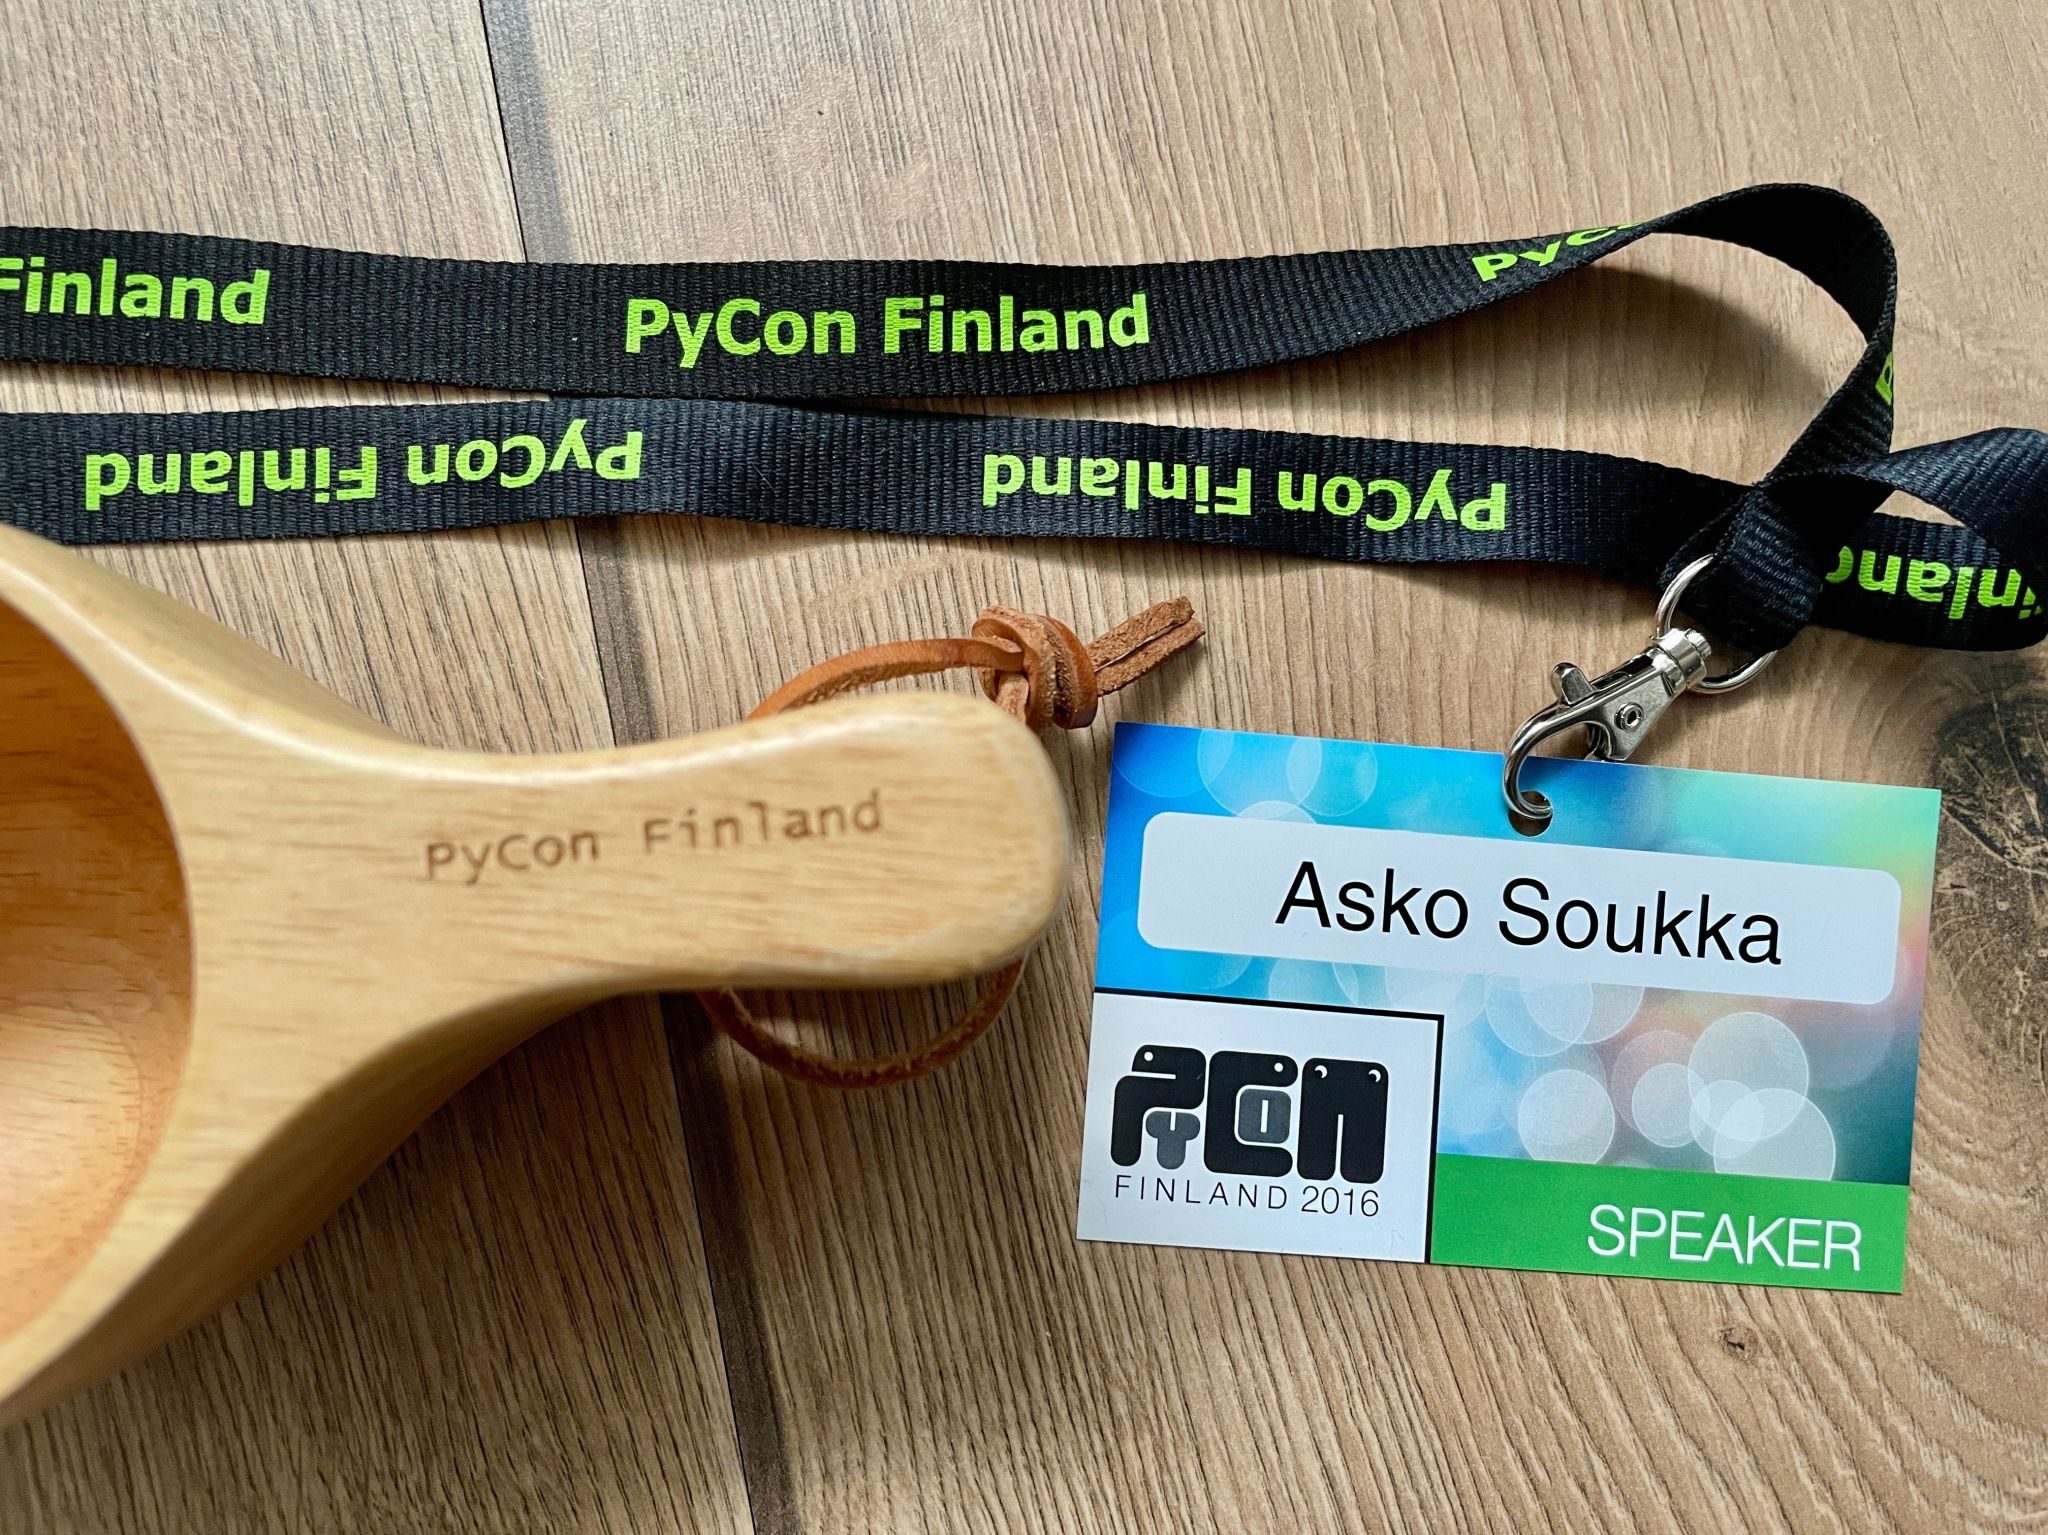
\includegraphics[width=\paperwidth, trim=0cm 0cm 0cm 5cm, clip]{images/pycon2016.jpg}
}
\begin{frame}[plain]
\end{frame}
}

%---------------------------------------------------------------------------------------

\setbeamertemplate{background canvas}[default]
\begin{frame}
\vfill
\centering \huge \textbf{PyCon Finland}
\par
\centering 
\includegraphics[height=0.50\paperheight]{images/PyCon-Finland.pdf}
\par
\textbf{Friday, October 17th 2025}
\vfill
\end{frame}

%---------------------------------------------------------------------------------------

\setbeamertemplate{background canvas}[default]
\begin{frame}
  \begin{minipage}{0.58\textwidth}
    \centering
    \huge \textbf{University of Jyväskylä}
    \par
    \vspace{0.5cm}
    \normalsize
    Python in production since 2003
  \end{minipage}
  \begin{minipage}{0.4\textwidth}
    \centering
    \vfill
    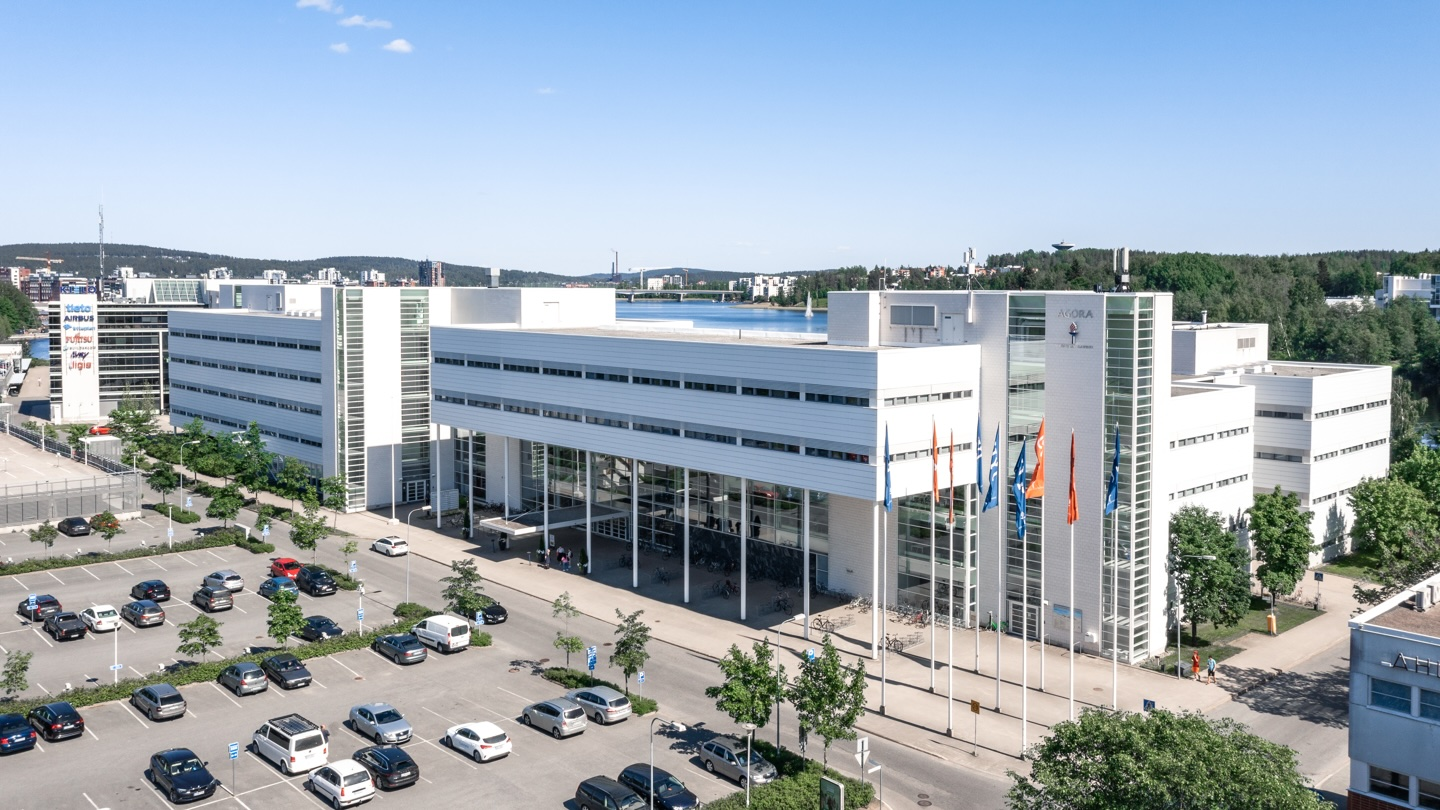
\includegraphics[height=\paperheight, trim=6cm 0cm 0cm 0cm, clip]{images/venue.jpg}
    \vfill
  \end{minipage}
\end{frame}
%---------------------------------------------------------------------------------------

\setbeamertemplate{background canvas}[default]
\begin{frame}
  \begin{minipage}{0.48\textwidth}
    \textbf{Plone Conference 2025}
    \begin{itemize}
      \item Mon-Sun, October 13th–19th
      \item Trainings, Conference, Sprint
      \item 200 international participants
      \item[]
      \item[]
      \item[]
      \item[]
    \end{itemize}
  \end{minipage}
  \hfill
  \begin{minipage}{0.48\textwidth}
    \only{\textbf{PyCon Finland 2025}}
    \begin{itemize}
      \item Friday, October 17th
      \item Tickets: 80 / 100 EUR
      \item Guaranteed audience
      \item International networking
      \item[]
      \item[] \small Limited capacity (\textasciitilde 100)
      \item[] \small Speakers for early bird rate
    \end{itemize}
  \end{minipage}
\end{frame}


%---------------------------------------------------------------------------------------

{
\setbeamertemplate{background}{
    
\includegraphics[width=\paperwidth, trim=0cm 0cm 0cm 0cm, clip]{images/rfjm.png}
}
\begin{frame}[plain]
\end{frame}
}

%---------------------------------------------------------------------------------------

\setbeamertemplate{background canvas}[default]
\begin{frame}
\vfill
\huge
\centering 
\includegraphics[height=0.50\paperheight]{images/PyCon-Finland.pdf}
\par
\textbf{\href{https://pyconfi.ploneconf.org}{fi.pycon.org}}
\par
\normalsize
\vfill
PyCon Finland 2025 – Friday, October 17th – Jyväskylä \\
Call for Proposal open – Early Bird Tickets available
\vfill
\end{frame}

%---------------------------------------------------------------------------------------

\end{document}
